\documentclass{../Vorlage/mat}
\lstset{
	basicstyle=\small
}

\begin{document}
\maketitle{Sebastian Bliefert}{}{Nils Drebing}{}{Pascal Pieper}{}{15.12.2016}{Bonus} \\

\section*{Aufgabe A}
\begin{align*}
\Phi & = 2 \pi \cdot \frac{47^{\circ}}{360^{\circ}}\\
& = 0.820304748437 
\end{align*}

\subsection*{a}
\begin{align*}
z & = exp(\imath \cdot \Phi)\\
& = cos(\Phi) + sin(\Phi)i\\
& = cos(0.820304748437) + sin(0.820304748437)i\\
z & = 0.681998360062 + 0.731353701619i
\end{align*}
\newpage

\subsection*{b}
\begin{figure}[!htb]
\centering
	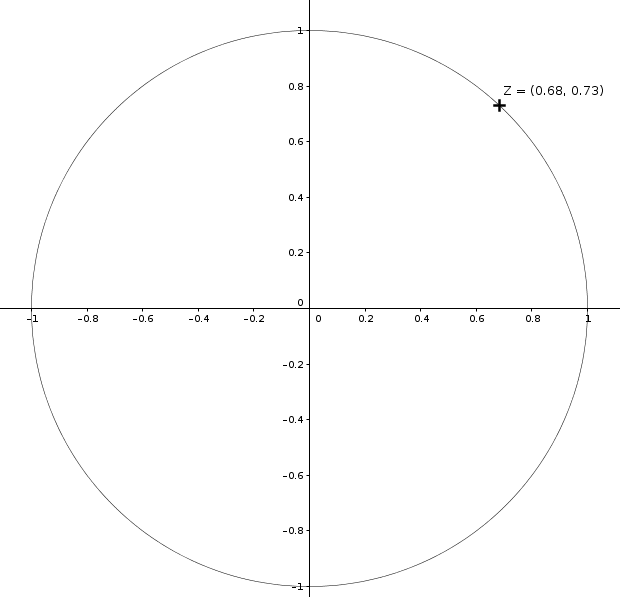
\includegraphics[scale=0.5]{circle_z.png}
	\label{circlez}
	\caption{Einheitskreis mit dem berechneten Punkt \textit{z}}
\end{figure}
\newpage

\subsection*{c}
\begin{figure}[!htb]
\centering
	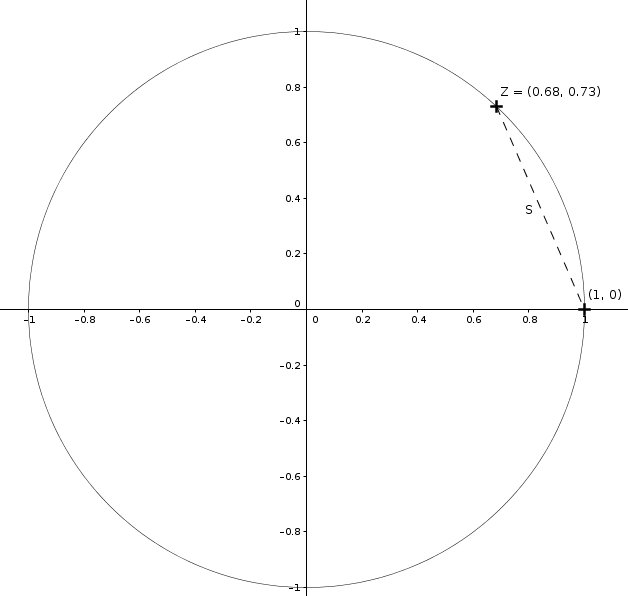
\includegraphics[scale=0.5]{circle_s.png}
	\label{circles}
	\caption{Einheitskreis mit dem berechneten Punkt \textit{z} und Strecke \textit{s} zwischen \textit{z} und $(1,0)^T$}
\end{figure}

\subsection*{d}
Nach Euklidischer Norm:
\begin{align*}
\|s\| & = \sqrt{(z_x - 1)^2 + (z_y - 0)^2}\\
& = \sqrt{(0.681998360062 - 1)^2 + 0.731353701619^2}\\
& = 0.79749813785
\end{align*}

\section*{Aufgabe B}


\section*{Aufgabe C}


\section*{Aufgabe D}


\end{document}
